\begin{boxD}
    در این تمرین ابتدا می‌بایستی به پیش‌پردازش مجموعه‌داده بپردازیم ، سپس با استفاده از منطق احتمال‌شرطی بیز به محاسبه میزان تعلق هر یک داده‌ها به هر کدام از کلاس‌ها خواهیم‌پرداخت.

\end{boxD}

\begin{boxD}
    \lr{Naive Bayes}
    یک مدل خاص از احتمال شرطی می‌باشد که این فرض را درنظرمی‌گیرد ، که همه ویژگی‌ها 
    \lr{feature}
    از یکدیگر مستقل هستند.

    تفاوت اصلی میان
    \lr{Naive Bayes}
    و طبقه‌بندی بیزی در همین استقلال ویژگی‌ها از یکدیگر است.

    زمانی بهتراست از این مدل‌ها استفاده کنیم که شرط استقلال 
    \lr{feature}
    از یکدیگر درست باشند.

    همچنین اگر تعداد ابعاد زیاد باشد و کارایی در محاسبات بسیارمهم است.

    زمانی که استقلال میان ویژگی‌ها برقرار نیست ، استفاده از این مدل هزینه زیادی دارد.

    این مدل معروف به مدل
    \lr{high bias low variance}
    می‌باشد.
\end{boxD}


\begin{figure}[h]
    \centering
    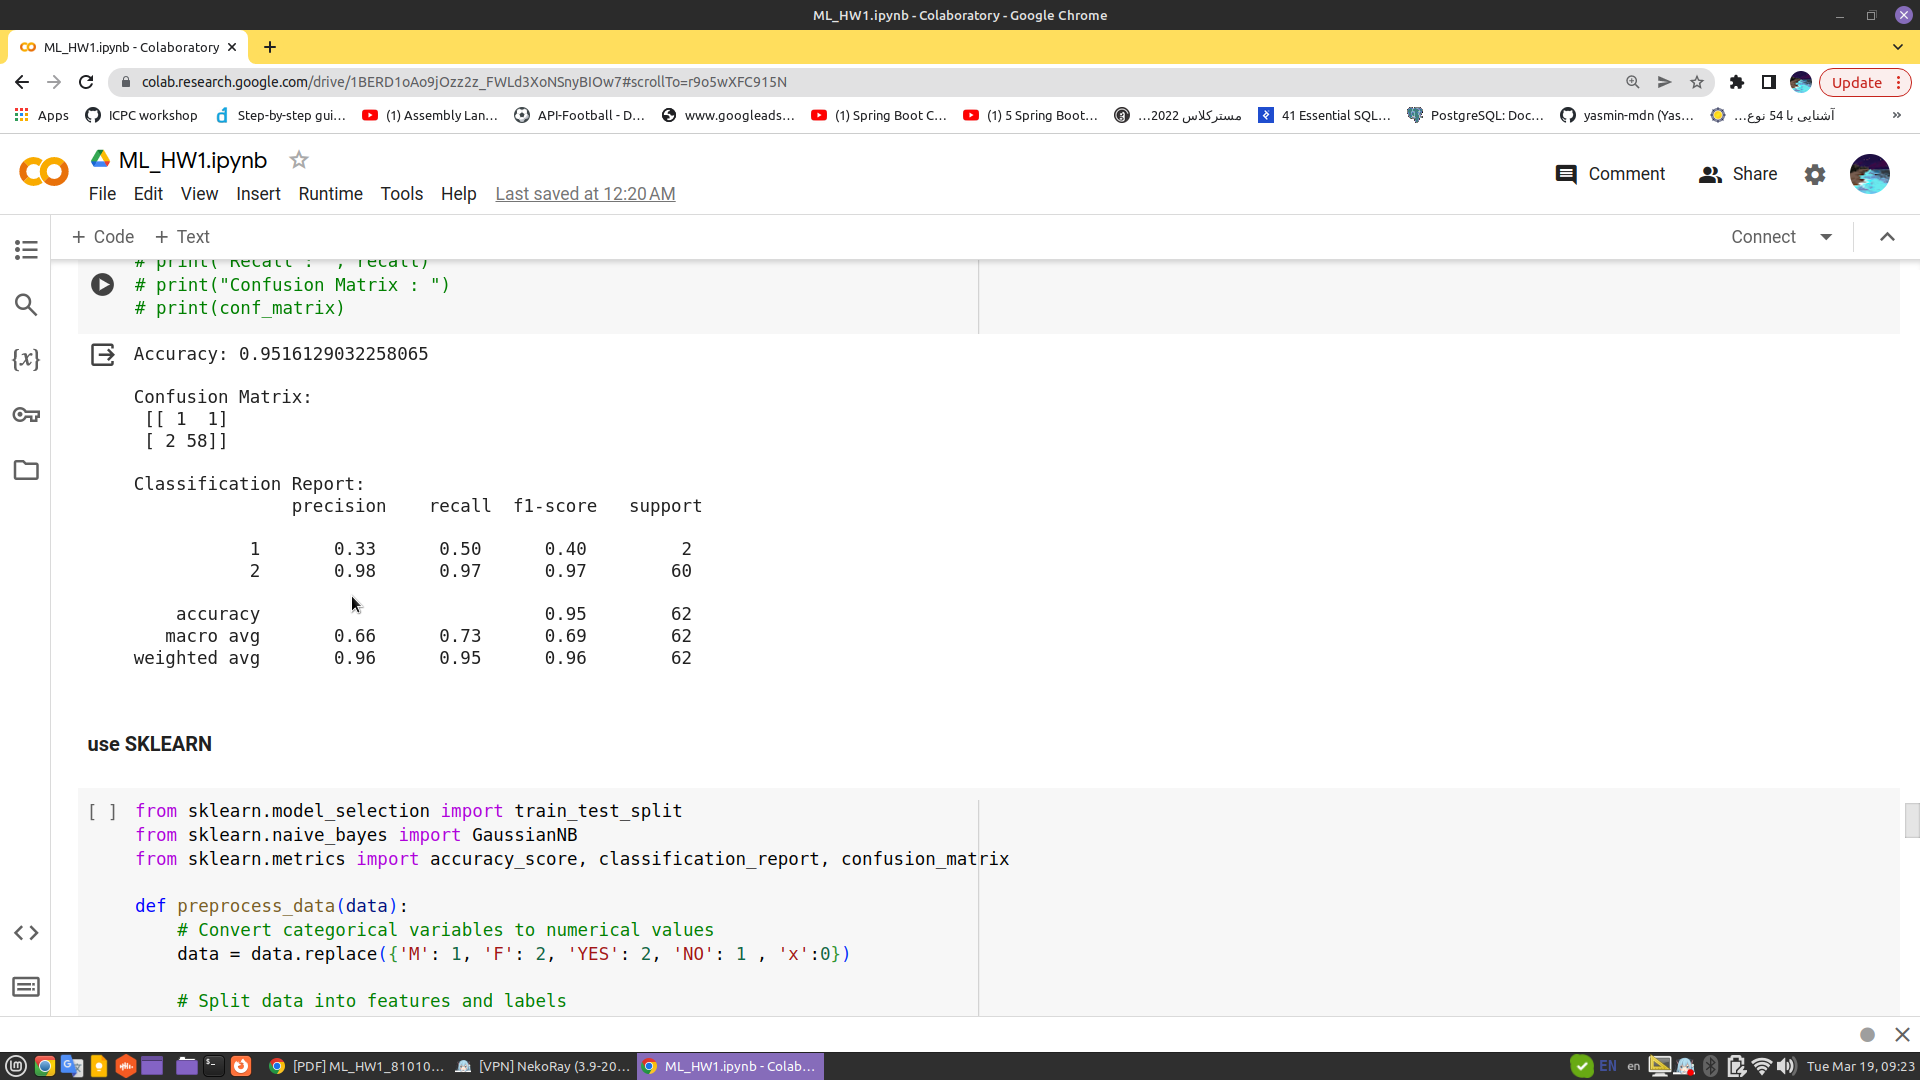
\includegraphics
    [width = 0.8\textwidth]
    {ML1/images/7-lung-self}
    \caption{پیاده‌سازی بدون کتابخانه از نایوبیز برای مجموعه‌داده سرطان ریه}
    \label{fig:enter-label}
\end{figure}

\begin{figure}[h]
    \centering
    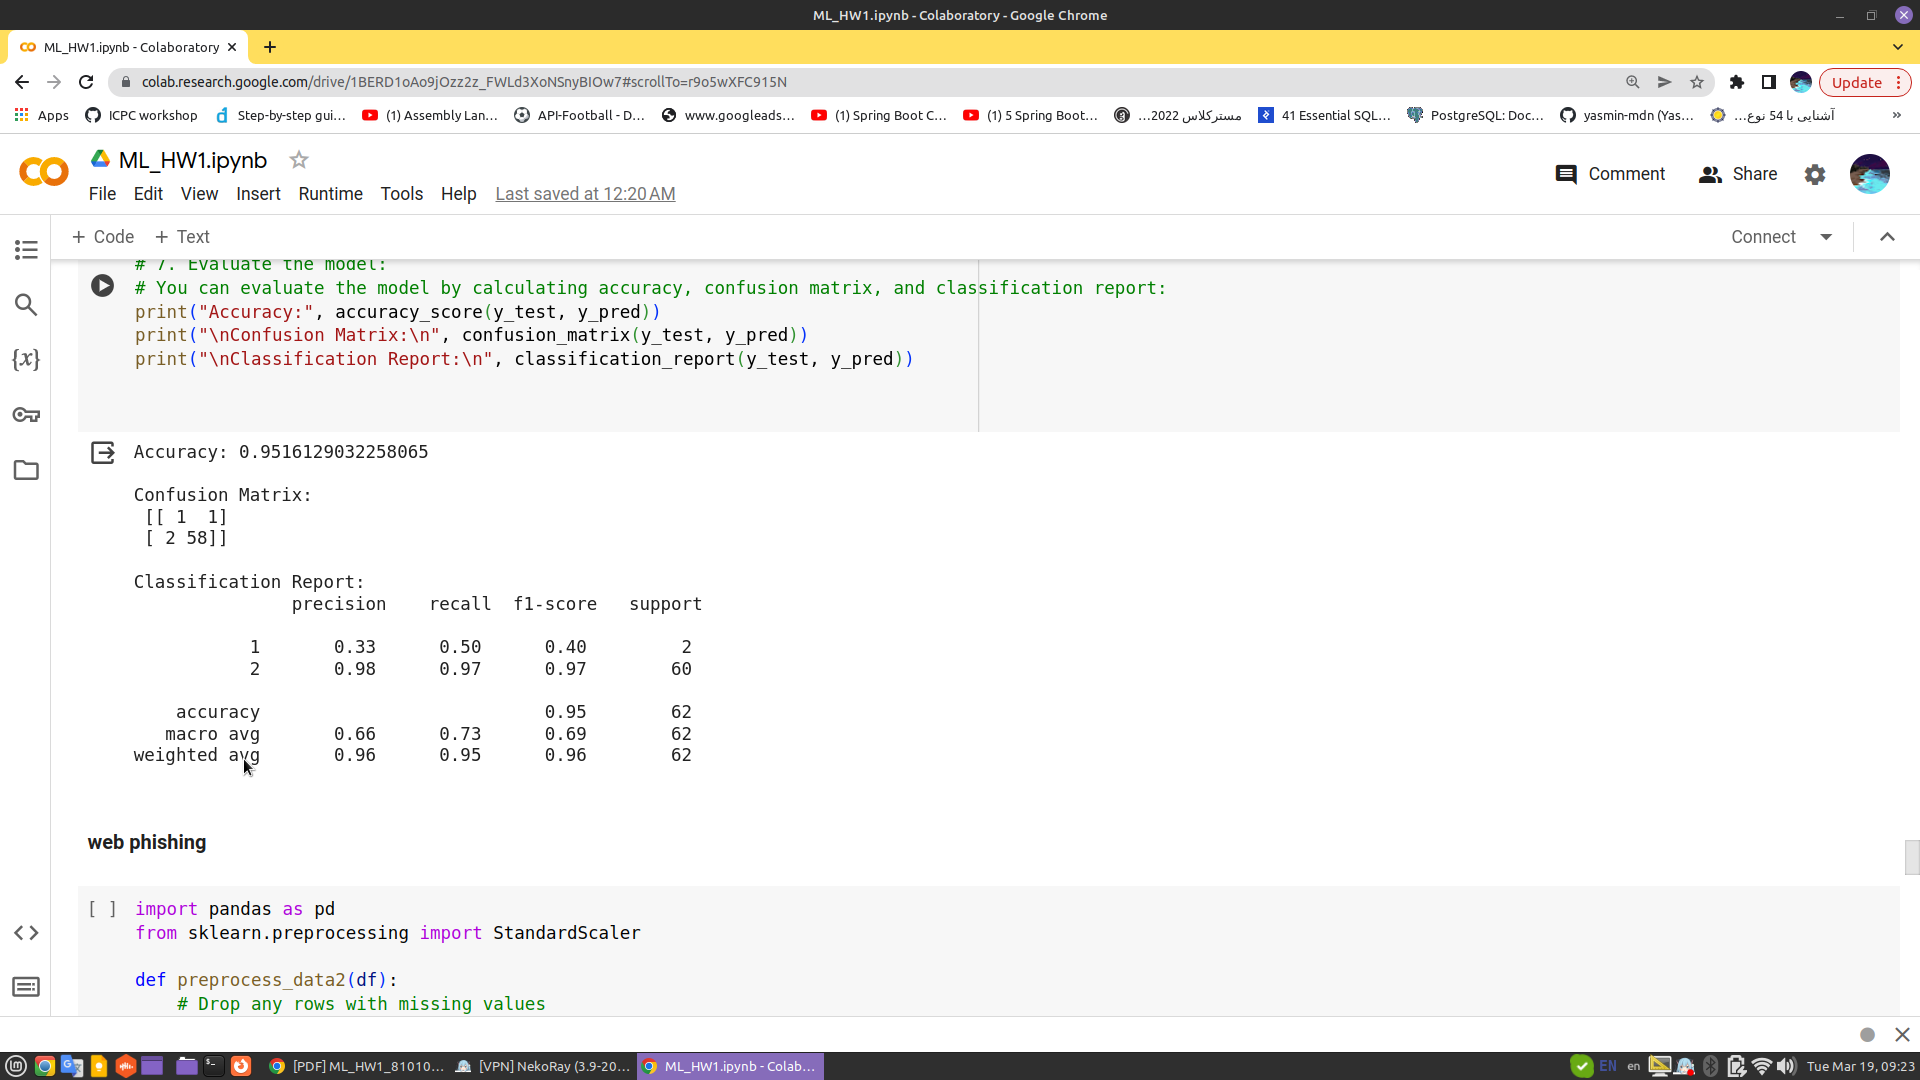
\includegraphics
    [width = 0.8\textwidth]
    {ML1/images/7-lung-sklearn}
    \caption{پیاده‌سازی 
    \lr{SKLEARN}
    از نایوبیز برای مجموعه‌داده سرطان ریه}
    \label{fig:enter-label}
\end{figure}

\begin{boxD}[h]
    برای پیش‌پردازش داده‌ها ابتدا کاراکترها را با یک معادل عددی جایگزین خواهیم‌کرد ، سپس به پیاده‌سازی مدل خواهیم پرداخت.
    برای پیاده‌سازی این مدل نیازمند 
    \lr{fit}
    کردن داده‌های آموزشی هستیم.

    در این تابع بایستی احتمال پیشین و احتمال
    \lr{likelihood}
    را محاسبه کنیم.

    سپس در تابع
    \lr{predict}
    به محاسبه 
    \begin{equation*}
        P(X | W_{1}) <> P(X | W_{2})
    \end{equation*}
    می‌پردازیم .
    هر کدام که مقدار بیشتری داشت را به عنوان برچسب کلاس انتخاب‌خواهیم‌کرد.

    می‌بینیم که این مدل مشابه پیاده‌سازی 
    \lr{SKLEARN}
    به محاسبه ماتریس آشفتگی می‌پردازد.
    تقریبا تفاوتی میان مدل‌ما و مدل پیش‌ساخته
    \lr{SKLEARN}
    وجود ندارد.
\end{boxD}

\begin{figure}[h]
    \centering
    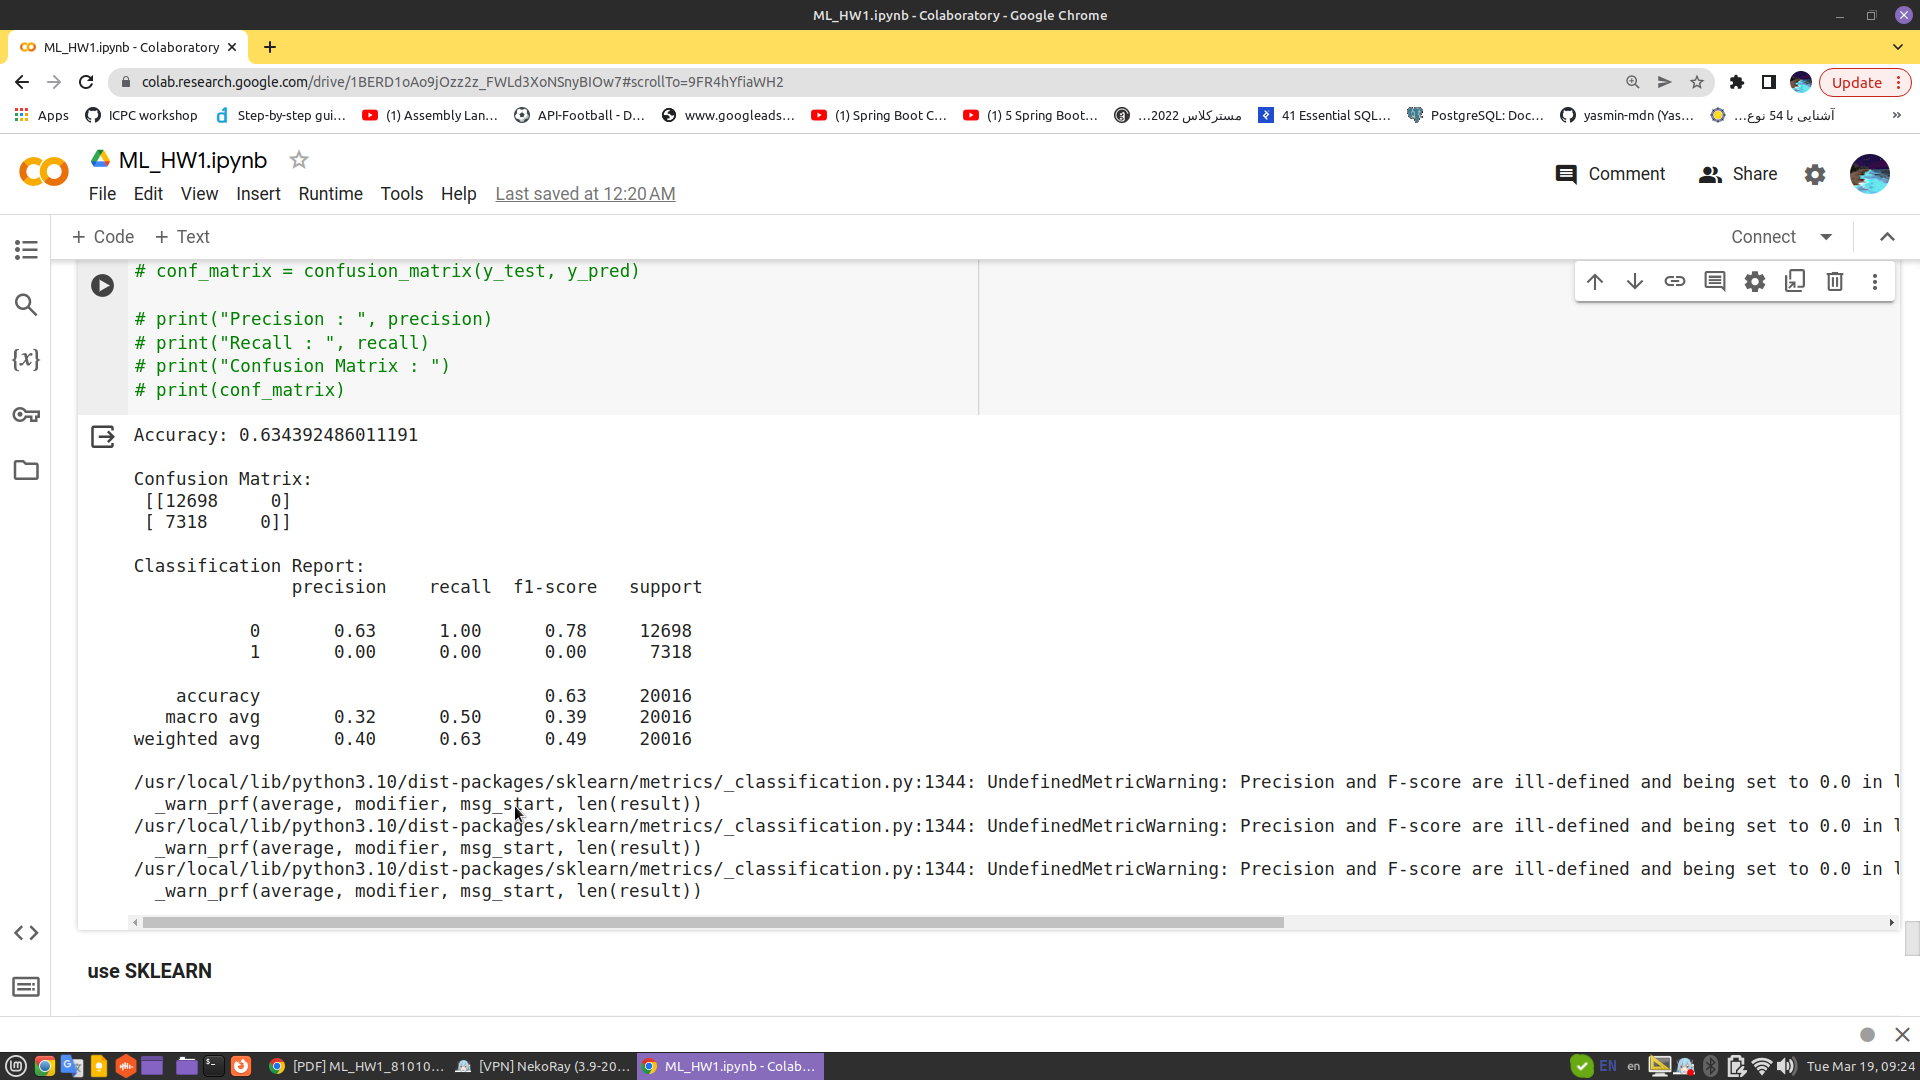
\includegraphics
    [width = 0.8\textwidth]
    {ML1/images/7-web-self}
    \caption{پیاده‌سازی بدون کتابخانه از نایوبیز برای مجموعه‌داده وب }
    \label{fig:enter-label}
\end{figure}

\begin{figure}[h]
    \centering
    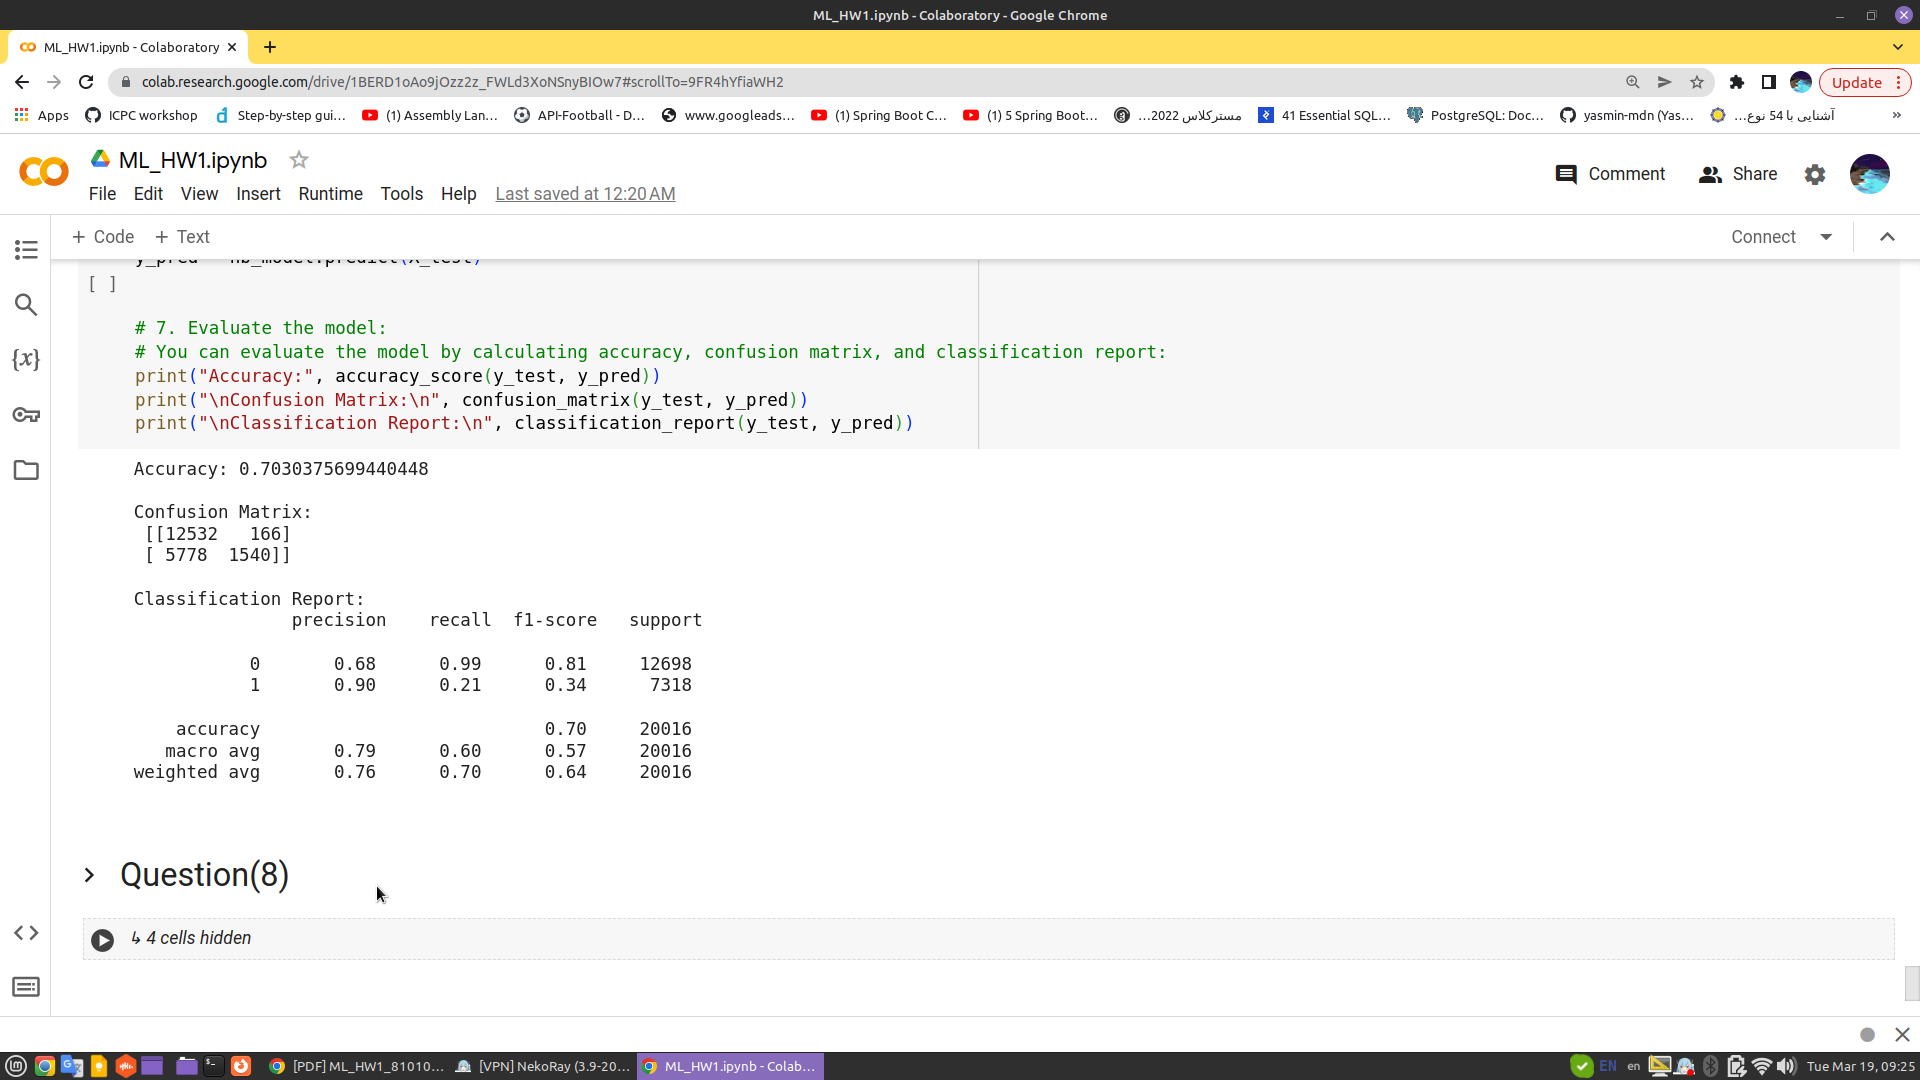
\includegraphics
    [width = 0.8\textwidth]
    {ML1/images/7-web-sklearn}
    \caption{پیاده‌سازی 
    \lr{SKLEARN}
    از نایوبیز برای مجموعه‌داده وب }
    \label{fig:enter-label}
\end{figure}

\begin{boxD}
    حال به بررسی مجموعه داده دوم خواهیم پرداخت . 
    این مجموعه داده ، بر خلاف مجموعه‌داده‌ قبلی دارای ویژگی‌هابا مقادیر پیوسته می‌باشد.

    همانطور که از مقایسه دقت‌ها نیز مشخص است ، دقت مدل ما با اختلاف فاحشی کمتر از مدل پیش‌ساخته 
    \lr{SKLEARN}
    می‌باشد.

    به نظر می‌رسد که دقت مدل ما در تخمین احتمالات 
    \lr{Likelihood}
    دقت کمتری نسبت به مدل پیش‌ساخته
    \lr{SKLEARN}
    دارد.
    علت این امر می‌تواند ناشی از چند عامل باشد .

    از مرحله پیش‌پردازش می‌توان گذر کرد چرا که هر دو روش را با یک تابع پیش‌پردازش و نرمال‌سازی کرده‌ایم.

    شاید داده‌ها بر روی داده آموزشی 
    \lr{overfit}
    شده باشد در مدلی که ما ساخته‌ایم.
    
\end{boxD}